\documentclass[10pt, a4paper]{article}

% various packages and settings {{{

% math packages
\usepackage{amsmath, amsfonts, mathtools}

% other important packages (should stay on top)
\usepackage{graphics, multicol, xcolor}

% change to German
\usepackage[german]{babel}

% utf8 characters
\usepackage[utf8]{inputenc}

% font
\usepackage[scaled]{helvet}
\renewcommand{\familydefault}{\sfdefault}
\usepackage[]{fontspec}

% fontsize
\usepackage[12pt]{extsizes}

% no paragraph indents
\setlength{\parindent}{0pt}

% better hyphenation
\usepackage[final]{microtype}
\usepackage{csquotes}

% import line spacing
\usepackage{setspace}

% page format
\usepackage{geometry}
\geometry{
    a4paper,
    left=25mm,
    right=25mm,
    top=15mm,
    bottom=25mm
}

% colorful boxes
\usepackage{mdframed}

\setcounter{secnumdepth}{0} % no section numbering
% }}}

% custom commands {{{
\usepackage{environ}

% define custom formula environment
\NewEnviron{formulas}{
    \vspace{-2.5em}
    \Large
    \begin{align*}
        \BODY
    \end{align*}
    \normalsize
}

% same formula env, but with red border
\NewEnviron{Formulas}{
    \begin{mdframed}[linecolor=red]
        \vspace{-2.5em}
        \Large
        \begin{align*}
            \BODY
        \end{align*}
        \normalsize
    \end{mdframed}
}

% normal-sized text inside the formulas
\newcommand{\normaltext}[1]{
    \normalsize\text{#1}\Large
}

% }}}

% set title spacing
\usepackage{titlesec}
\titlespacing\section{0pt}{12pt}{0pt}
\titlespacing\subsection{0pt}{12pt}{0pt}
\titlespacing\subsubsection{0pt}{12pt}{0pt}

% position tables
\usepackage{float}

% binary trees
\usepackage[edges]{forest}

% no caption enumeration
\usepackage{caption}
\captionsetup{labelformat=empty}

\begin{document}

\addtocounter{page}{-3}
\setstretch{1.5}

\title{Informatik 12/13 Niedersachsen}
\date{\today}

\maketitle

\thispagestyle{empty}

\clearpage

\thispagestyle{empty}

\tableofcontents

\thispagestyle{empty}

\clearpage

% ------------ Vektoren, Geraden, Ebenen, Abstände im Raum ------------ %
\section{Datenstrukturen}

Datenstrukturen dienen der strukturierten Speicherung von Daten, meist im Arbeitsspeicher.
Es soll schneller Zugriff und dass einfache Anwendungen von Algorithmen ermöglicht werden,
wobei es wichtig ist, dass die Datenstruktur zu den Daten passt.
Alle Beschreibungen der Datenstrukturen beziehen sich auf die Vorgaben des
Kerncurriculums Informatik.

\subsection{Statische Reihung}

Die statische Reihung (vgl. Array) speichert Daten eines Datentyps und hat
eine feste Länge. Der Zugriff auf die Daten erfolgt indexbasiert und
mit einer Zugriffszeit von $O(1)$.

\subsection{Dynamische Reihung}

\begin{table}[H]
    \begin{tabular}{|p{0.50\linewidth}|p{0.50\linewidth}|}
    \hline
    DynArray(): DynArray & Eine leere dynamische Reihung wird angelegt. \\ \hline
    isEmpty(): Wahrheitswert & Gibt True zurück, wenn die Reihung leer ist. \\ \hline
    getItem(Ganzzahl index): Inhalt & Gibt das Element am Index zurück. \\ \hline
    append(Inhalt inhalt) & Fügt ein Element am Ende hinzu. \\ \hline
    insertAt(Ganzzahl index, Inhalt inhalt) & Fügt ein Element am Index ein. Die Elemente rechts davon rücken um 1 Position nach rechts. \\ \hline
    setItem(Ganzzahl index, Inhalt inhalt) & Ersetzt das Element am Index. \\ \hline
    delete(Ganzzahl index) & Löscht das Element am Index, die anderen Elemente rücken nach links. \\ \hline
    getLength(): Ganzzahl & Gibt die Länge zurück \\ \hline
    \end{tabular}
\end{table}
























\subsection{Schlange}
\subsection{Stapel}
\subsection{Binärbaum}
\subsubsection{Traversierung von Binärbäumen}
\subsubsection*{Pre-Order}
\subsubsection*{In-Order}
\subsubsection*{Post-Order}

\section{Rekursive Problemlösung}

\subsection{Divide and Conquer Prinzip}

Beim ``Divide and Conquer'' (Teile und Herrsche) Prinzip wird ein größeres, schwereres Problem
in viele Kleine zerlegt, die dann jedes für sich einfacher gelöst werden können.
Dies geschieht häufig mit rekursiven Funktionen z. B. bei Such- und Sortierverfahren
(e.g. Binäre Suche, Quicksort).

\subsection{Fachbegriffe der Rekursion}

\subsubsection{Abbruchbedingung (Rekursionsanker)}

Die Abbruchbedingung verhindert die unendliche Ausführung der rekursiven Funktion.
Sie stellt dabei die Basis der rekursiven Definition dar und wird meist nach dem vollständigen
rekursiven Abstieg erreicht.

\begin{lstlisting}
sum(n)
    if n=0 # Rekursionsanker
        return 0
    else    # Rekursionsabstieg
        return n + sum(n-1)
\end{lstlisting}

\subsubsection{Rekursiver Abstieg/Aufstieg}
\label{sec:rekursion_ab_auf}

Der rekursive Abstieg bezeichnet das rekursive Selbstaufrufen der Funktion bis zum
erreichen des Rekursionsankers. Danach beginnt der Rekursionsaufstieg, bei dem
das Ergebnis berechnet bzw. zurückgegeben wird.

\begin{lstlisting}
sum(3) = 3 + sum(2)             # Beginn Rekursiver Abstieg
    sum(2) = 2 + sum(1)
        sum(1) = 1 + sum(0)
            sum(0) = 0          # Auslösen Rekursionsanker
        sum(1) = 1 + 0 = 1
    sum(2) = 2 + 1 = 3
sum(3) = 3 + 3 = 6              # Ende Rekursiver Aufstieg
\end{lstlisting}


\subsection{Rekursionsarten}

\subsubsection{Aufsteigende Rekursion (Einzelrekursion)}

Bei der Aufsteigenden Rekursion wird das Ergebnis der rekursiven Funktion
beim Rekursionsaufstieg berechnet. Dies ist beispielhaft bei \hyperref[sec:rekursion_ab_auf]{Rekursiver Abstieg/Aufstieg} beschrieben.

\begin{lstlisting}
sum(n)
    if n=0
        return 0
    else
        return n + sum(n-1)
\end{lstlisting}

\subsubsection{Endrekursion (Einzelrekursion)}

Bei der Endrekursion erfolgt die Berechnung beim Rekursionsabstieg und endet,
wenn die Abbruchbedingung erreicht ist. Beim Rekursionsaufstieg wird nur das
Ergebnis durchgereicht.

\begin{lstlisting}
sum(m, n)
    if n=0
        return m
    else
        return sum(m+n, n-1)
\end{lstlisting}

\subsubsection{Baumartige Rekursion (Mehrfachrekursion)}

Bei der Baumartigen bzw. Kaskadierenden Rekursion ruft sich eine Funktion pro Funktionsaufruf
mehrmals rekursiv auf. Der Rückgabewert setzt sich aus der Kombination 2er oder mehr Aufrufe
der Funktion zusammen.

\begin{lstlisting}
bintree_sum(t)
    if t.leaf()
        return t.value()
    else
        return bintree_sum(t.left()) + bintree_sum(t.right())
\end{lstlisting}

\subsubsection{Weitere Rekursionsarten (Nicht Kerncurriculum relevant)}

Indirekte Rekursion bezeichnet 2 oder mehr Funktionen, die sich zwar
nicht direkt selbst sondern gegenseitig aufrufen, wodurch auch Rekursion
zustande kommen kann.

\begin{lstlisting}
f(x)
    ...
    return g(x - 1)

g(x)
    ...
    return f(x - 1)
\end{lstlisting}

Geschachtelte Rekursion bezeichnet die Schachtelung von rekursiven Aufrufen
innerhalb der Funktion.

\begin{lstlisting}
f(x)
    ...
    return f(x - f(x))
\end{lstlisting}

\section{Algorithmen}

\subsection{Binäre Suche}

Die Binäre Suche ist ein Algorithmus um in sortierten Datenstrukturen (z. B. Reihungen)
ein Element zu finden. Dabei werden maximal $log_{2}(n) + 1$ Operationen benötigt,
bis das Element gefunden wird (oder feststeht, das es nicht enthalten ist).
Die Binäre Suche lässt sich auf lexikographisch sortierbare Datentypen anwenden,
z. B. eine Reihung von Ganzzahlen. Durch vergleichen des gesuchten Werts mit dem mittleren
Wert des aktuellen Bereiches kann festgestellt werden, ob sich dieser Wert im linken oder
rechten Teil des sortierten Bereichs befindet. Anschließend wird mit dem mittleren Wert
des neuen Teilbereichs verglichen und schließlich findet man so das gesuchte Element.
Durch jeden Vergleich wird der Suchbereich halbiert und die nötigen Vergleiche sind
logarithmisch zur Elementanzahl.

\vspace*{0.3cm}
Es soll geprüft werden, ob die Zahl 2 in der sortierten Reihung enthalten ist.
Der aktuelle Vergleich (mittleres Element) ist rot und der aktuelle Bereich blau markiert.
Nach 4 Vergleichen ist klar, dass 2 enthalten ist. 
Es wurden also $log_{2}(11) + 1$ Versuche benötigt.

% matrix magic
\pgfdeclarelayer{myback}
\pgfsetlayers{myback,background,main}

\tikzset{mycolor/.style = {line width=1bp,color=#1}}%
\tikzset{myfillcolor/.style = {draw,fill=#1}}%

\NewDocumentCommand{\highlight}{O{blue!40} m m}{%
\draw[mycolor=#1] (#2.north west)rectangle (#3.south east);
}

\begin{figure}[H]
    \centering
    \adjustbox{scale=1.5}{
        \begin{tikzpicture}[baseline=-\the\dimexpr\fontdimen22\textfont2\relax ]
        \matrix (m) [
            matrix of math nodes,
            left delimiter={[},
            right delimiter={]},
            row sep=10pt,
            r/.style={fill=red!20},
            b/.style={fill=blue!20}
        ] {
            1 & 2 & 3 & 4 & 5 & |[r]| 6 & 7 & 8 & 9 & 10 & 11 \\
            1 & 2 & |[r]| 3 & 4 & 5 & 6 & 7 & 8 & 9 & 10 & 11 \\
            |[r]| 1 & 2 & 3 & 4 & 5 & 6 & 7 & 8 & 9 & 10 & 11 \\
            1 & |[r]| 2 & 3 & 4 & 5 & 6 & 7 & 8 & 9 & 10 & 11 \\
        };
        
        \begin{pgfonlayer}{myback}
        \highlight[blue]{m-1-1}{m-1-11}
        \highlight[blue]{m-2-1}{m-2-5}
        \highlight[blue]{m-3-1}{m-3-2}
        \highlight[blue]{m-4-2}{m-4-2}
        \end{pgfonlayer}
        \end{tikzpicture}
    }
\end{figure}

\clearpage

\subsection{Quicksort}

Quicksort ist ein von Tony Hoare publizierter, rekursiver Sortieralgorithmus mit einer
Komplexität von $O(n \cdot log_{2}(n))$, von dem viele unterschiedlich gute Variationen existieren.
Die Grundstruktur aller Versionen ist dabei ähnlich.

\begin{enumerate}
    \item Wenn die Länge des Sortierbereichs kleiner als 2 ist, ist der Bereich sortiert.
    Es kann auch bei anderen Minimalgrenzen (e.g. 10) dann der Bereich mit einem anderen
    Algorithmus sortiert werden.
    \item Ist dies nicht der Fall, wird ein Pivot Element ausgewählt. Dabei gibt es Verschiedene
    Wege der Auswahl (z. B. kann man das Mittlere nehmen).
    \item Anschließend wird der Sortierbereich in 2 Unterbereiche aufgeteilt, sodass in einem
    Bereich alle Elemente kleiner oder gleich und im anderen Bereich alle Elemente größer oder gleich
    dem Pivot Element sind.
    \item Anschließend wendet man Quicksort (Schritte 1 bis 4) auf jeden dieser Unterbereich an.
\end{enumerate}

Ein auf Hoares Publikation beruhender Pseudocode könnte wie folgt aussehen.
Die Funktion $quicksort$ sorgt für das Anwenden der Partitionsmethode und das rekursive
Aufrufen. Hoares Partitionsfunktion nutzt in $partition$ 2 Zeiger, einer startet links,
der andere rechts. Der Linke bewegt sich nach rechts, solange alle Elemente kleiner
als das Pivot Element sind. Der Rechte bewegt sich nach links, solange alle Elemente
größer als das Pivot Element sind. Wenn beide Zeiger stoppen und sie sich nicht überkreuzt
haben, so sind jeweils die Elemente an der Zeigerposition im falschen Teil des Bereichs und
müssen getauscht werden. Durch Wiederholung wird so der Bereich in die für Quicksort gewollten
2 Bereiche geteilt. Die Trennung der Bereiche liegt dort, wo sich die Zeiger begegnen.

\begin{figure}[H]
\begin{lstlisting}
algorithm quicksort(A, lo, hi) is 
    if lo >= 0 && hi >= 0 && lo < hi then
        b := partition(A, lo, hi) // b is r at the end of partition()
        quicksort(A, lo, b)
        quicksort(A, b + 1, hi) 

algorithm partition(A, lo, hi) is 
    pivot := A[ floor((hi - lo)/2) + lo ] // middle of array

    l := lo - 1
    r := hi + 1

    loop forever 
        do l := l + 1 while A[l] < pivot
        do r := r - 1 while A[r] > pivot

        if l >= r then return r

        swap A[l] with A[r]
\end{lstlisting}
\caption{\textbf{Pseudocode für Quicksort nach Hoare}}
\end{figure}

\begin{figure}[H]
\begin{lstlisting}[language=python]
def quicksort(array, lo, hi):
    if lo >= 0 and hi >= 0 and lo < hi:
        b = partition(array, lo, hi)
        quicksort(array, lo, b)
        quicksort(array, b + 1, hi)


def partition(array, lo, hi):
    pivot = array[int((hi - lo) / 2) + lo]

    l = lo - 1
    r = hi + 1

    while True:
        l += 1
        while arrray[l] < pivot:
            l += 1
        
        r += 1
        while arrray[r] < pivot:
            r += 1

        if l >= r:
            return r

        temp = array[l]
        array[l] = array[r]
        array[r] = temp
\end{lstlisting}
\caption{\textbf{Python Code für Quicksort nach Hoare}}
\end{figure}

\begin{figure}[H]
    % \centering
    \adjustbox{scale=1.2}{
        \begin{tikzpicture}[baseline=-\the\dimexpr\fontdimen22\textfont2\relax]
        \matrix (m) at (0,0) [
            matrix of math nodes,
            left delimiter={[},
            right delimiter={]},
            row sep=10pt,
            r/.style={fill=red!20},
            b/.style={fill=blue!20},
            g/.style={fill=green!20},
            v/.style={fill=violet!20},
            yl/.style={fill=yellow!20},
            row 11 column 4/.style={ nodes = { top color=violet!50, bottom color=green!30 }},
            row 17 column 2/.style={ nodes = { top color=violet!50, bottom color=green!30 }},
            row 19 column 5/.style={ nodes = { top color=violet!50, bottom color=green!30 }}
        ] {
           1 & 8 & 10 & 6 & 7 & 5 & 9 & [1em] |[r]| 6 \\
           |[v]| 1 & 8 & 10 & 6 & 7 & 5 & 9 & [1em] |[r]| 6 \\
           1 & |[v]| 8 & 10 & 6 & 7 & 5 & 9 & [1em] |[r]| 6 \\
           1 & |[v]| 8 & 10 & 6 & 7 & 5 & |[g]| 9 & [1em] |[r]| 6 \\
           1 & |[v]| 8 & 10 & 6 & 7 & |[g]| 5 & 9 & [1em] |[r]| 6 \\
           1 & |[yl]| 5 & 10 & 6 & 7 & |[yl]| 8 & 9 & [1em] |[r]| 6 \\
           1 & 5 & |[v]| 10 & 6 & 7 & |[g]| 8 & 9 & [1em] |[r]| 6 \\
           1 & 5 & |[v]| 10 & 6 & |[g]| 7 & 8 & 9 & [1em] |[r]| 6 \\
           1 & 5 & |[v]| 10 & |[g]| 6 & 7 & 8 & 9 & [1em] |[r]| 6 \\
           1 & 5 & |[yl]| 6 & |[yl]| 10 & 7 & 8 & 9 & [1em] |[r]| 6 \\
           1 & 5 & 6 & 10 & 7 & 8 & 9 & [1em] |[r]| 6 \\
           1 & 5 & |[g]| 6 & |[v]| 10 & 7 & 8 & 9 & [1em] |[r]| 6 \\
           1 & 5 & 6 & 10 & 7 & 8 & 9 & [1em] |[r]| 5 & [0.5em] |[r]| 7 \\
           |[v]| 1 & 5 & 6 & |[v]| 10 & 7 & 8 & 9 & [1em] |[r]| 5 & [0.5em] |[r]| 7 \\
           1 & |[v]| 5 & 6 & |[v]| 10 & 7 & 8 & |[g]| 9 & [1em] |[r]| 5 & [0.5em] |[r]| 7 \\
           1 & |[v]| 5 & |[g]| 6 & |[v]| 10 & 7 & |[g]| 8 & 9 & [1em] |[r]| 5 & [0.5em] |[r]| 7 \\
           1 & 5 & 6 & |[v]| 10 & |[g]| 7 & 8 & 9 & [1em] |[r]| 5 & [0.5em] |[r]| 7 \\
           1 & 5 & 6 & |[yl]| 7 & |[yl]| 10 & 8 & 9 & [1em] & [0.5em] |[r]| 7 \\
           1 & 5 & 6 & 7 & 10 & 8 & 9 & [1em] & [0.5em] |[r]| 7 \\
           1 & 5 & 6 & |[g]| 7 & |[v]| 10 & 8 & 9 & [1em] & [0.5em] |[r]| 7 \\
           1 & 5 & 6 & 7 & 10 & 8 & 9 & [1em] |[r]| 8 & [0.5em] \\
           \dots \\
           1 & 5 & 6 & 7 & 8 & 9 & 10 & [1em] & [0.5em] \\
        };
        \draw[thick,red] ([xshift=0.5em]m-1-7.north east) -- ([xshift=0.5em]m-23-7.south east);
        
        \begin{pgfonlayer}{myback}
            \highlight[blue]{m-1-1}{m-1-7}
            \highlight[blue]{m-2-1}{m-2-7}
            \highlight[blue]{m-3-1}{m-3-7}
            \highlight[blue]{m-4-1}{m-4-7}
            \highlight[blue]{m-5-1}{m-5-7}
            \highlight[blue]{m-6-1}{m-6-7}
            \highlight[blue]{m-7-1}{m-7-7}
            \highlight[blue]{m-8-1}{m-8-7}
            \highlight[blue]{m-9-1}{m-9-7}
            \highlight[blue]{m-10-1}{m-10-7}
            \highlight[blue]{m-11-1}{m-11-7}
            \highlight[blue]{m-12-1}{m-12-7}
            \highlight[blue]{m-13-1}{m-13-3}\highlight[blue]{m-13-4}{m-13-7}
            \highlight[blue]{m-14-1}{m-14-3}\highlight[blue]{m-14-4}{m-14-7}
            \highlight[blue]{m-15-1}{m-15-3}\highlight[blue]{m-15-4}{m-15-7}
            \highlight[blue]{m-16-1}{m-16-3}\highlight[blue]{m-16-4}{m-16-7}
            \highlight[blue]{m-17-1}{m-17-3}\highlight[blue]{m-17-4}{m-17-7}
            \highlight[green]{m-18-1}{m-18-1}\highlight[green]{m-18-2}{m-18-3}\highlight[blue]{m-18-4}{m-18-7}
            \highlight[green]{m-19-1}{m-19-1}\highlight[green]{m-19-2}{m-19-3}\highlight[blue]{m-19-4}{m-19-7}
            \highlight[green]{m-20-1}{m-20-1}\highlight[green]{m-20-2}{m-20-3}\highlight[blue]{m-20-4}{m-20-7}
            \highlight[green]{m-21-1}{m-21-1}\highlight[green]{m-21-2}{m-21-3}\highlight[green]{m-21-4}{m-21-4}\highlight[blue]{m-21-5}{m-21-7}
            \highlight[green]{m-23-1}{m-23-1}\highlight[green]{m-23-2}{m-23-3}\highlight[green]{m-23-4}{m-23-4}\highlight[green]{m-23-5}{m-23-5}\highlight[green]{m-23-6}{m-23-7}
        \end{pgfonlayer}
        
        \matrix (m) at (7, 0) [
            matrix of math nodes,
            left delimiter={[},
            right delimiter={]},
            row sep=10pt,
            r/.style={fill=red!20},
            g/.style={fill=green!20},
            v/.style={fill=violet!20},
            yl/.style={fill=yellow!20},
        ] {
            |[r]| 6 & [0.5em] \textnormal{Pivot Element} \\
            |[v]| 1 & \textnormal{Left Pointer} \\
            |[g]| 9 & \textnormal{Right Pointer} \\
            |[yl]| 5 & \textnormal{Swap Elements} \\
            3 & \textnormal{Sort Range} \\
            7 & \textnormal{Finished Range} \\
        };
        \begin{pgfonlayer}{myback}
            \highlight[blue]{m-5-1}{m-5-1}
            \highlight[green]{m-6-1}{m-6-1}
        \end{pgfonlayer}
        \end{tikzpicture}
    }
    \caption{\textbf{Beispieldurchlauf des Algorithmus}}
\end{figure}

\clearpage

\subsection{Trace-Tabellen}

Eine Trace Tabelle soll die Veränderung der Daten (Variablen)
während der Ausführung eines Programms (Algorithmus) darstellen
und ist vergleichbar mit einem Debugger.

\begin{figure}[H]
\begin{lstlisting}
int x;
for (i = 0; i < 3; i++){
    for(j = 0; j < 2; j++){
        x = i + j; 
        // trace here
    }
}
// trace here
\end{lstlisting}
\end{figure}

\begin{table}[H]
    \begin{tabular}{|l|l|l|}
    \hline
        i & j & x \\ \hline
        0 & 0 & 0 \\ \hline
        0 & 1 & 1 \\ \hline
        1 & 0 & 1 \\ \hline
        1 & 1 & 2 \\ \hline
        2 & 0 & 2 \\ \hline
        2 & 1 & 3 \\ \hline
        ? & ? & 3 \\ \hline
    \end{tabular}
\end{table}

\section{Codierung}

\subsection{Lauflängen-Codierung}

Die Lauflängenkodierung komprimiert verlustfrei längere Abfolgen gleicher Symbole.

\begin{lstlisting}
AAAAA => 5A
\end{lstlisting}

Sind bei einem Bild z. B. 100 Pixel, die aufeinander Folgen, weiß,
so muss nur noch 1 Pixel und die Anzahl gespeichert werden. Wenn 1 Pixel
24 Bit groß ist, werden so unfähr 2,4 Kilobyte eingespart.

\subsection{Huffman-Codierung}

Bei der Huffman Codierung wird die Gesamtlänge der Daten dadurch reduziert,
dass häufig vorkommende Symbole mit kürzeren Bitfolgen kodiert werden und
selten vorkommende Symbole mit längeren Bitfolgen. Dadurch lässt sich die Gesamtlänge
meist deutlich reduzieren. Je größer die Entropie der zu Kodierenden Symbole, desto
höher ist die Kompressionsrate.

Die resultierende Kodierung für eine Menge an Symbolen ist ein Präfixcode
(erfüllt Fano-Bedingung).
Das heißt, dass keine Bitfolge zur kodierung eines Symbols zu Beginn einer
anderen Bitfolge zu finden ist. Somit ist es immer klar möglich, die Bitfolge
einem Symbol zuzuordnen und festzustellen, wann die Bitfolge zuende ist.
Um die Huffmann-Kodierung praktisch zu nutzen, muss die Huffmann-Kodierung
zur decodierung allerdings immer mitgeliefert werden und verbraucht auch Platz.
Lohnenswert ist die Huffmann-Kodierung also nur, wenn die Einsparungen größer sind als
der Platz, den die Dekodierungstabelle verbraucht. 

\subsubsection{Erstellung einer Huffman-Kodierung}

Beim ASCII Code wird jedes Zeichen mit 8 Bit kodiert.
Für jeden bestimmten Text lässt sich allerdings eine auf diesen
zugeschnitte, meist bessere, Huffmann-Kodierung generieren.
Zuerst werden die Häufigkeiten der Zeichen bestimmt.

\begin{lstlisting}
ABACEADBCEEEC
A: 3
B: 2
C: 3
D: 1
E: 4
Gesamt: 13
\end{lstlisting}

\clearpage

Anschließend lässt sich die individuelle Kodierung über einen Huffmann-Baum erstellen.
Es werden alle Häufigkeiten als Knoten betrachtet. Dann wird folgendes solange
wiederholt, bis es nur noch 1 Baum gibt. Dabei können für Symbolfolgen auch
mehrere unterschiedliche aber alle valide Bäume entstehen.

\begin{enumerate}
    \item Wähle die Teilbäume mit der geringsten absoluten/relativen Häufigkeit in
    der Wurzel. Bei gleicher Häufigkeit wähle den Teilbaum mit der geringeren Tiefe.
    \item Fasse diese zu einem neuen Teilbaum zusammen, in dessen Wurzel die Summe
    der Häufigkeiten der Wurzeln der Teilbäume steht.
    (Teilbaum mit geringerer Häufigkeit möglichst immer auf der gleichen Seite für optimale Kodierung)
\end{enumerate}

\vspace*{0.5cm}

\begin{forest}
for tree={
    grow=south,
    circle, draw, minimum size=5ex, inner sep=3pt,
    s sep=7mm
}
[, phantom, s sep = 7mm
    [A: 3]
    [B: 2]
    [C: 3]
    [D: 1]
    [E: 4]
]
\end{forest}

\vspace*{1cm}

\begin{forest}
for tree={
    grow=south,
    circle, draw, minimum size=5ex, inner sep=3pt,
    s sep=7mm
}
[, phantom, s sep = 7mm
    [3
        [D: 1]
        [B: 2]
    ]
    [3, phantom, s sep = 7mm
        [A: 3]
        [C: 3]
        [E: 4]
    ]
]
\end{forest}

\vspace*{1cm}

\begin{forest}
for tree={
    grow=south,
    circle, draw, minimum size=5ex, inner sep=3pt,
    s sep=7mm
}
[, phantom, s sep = 7mm
    [6
        [A: 3]
        [3
            [D: 1]
            [B: 2]
        ]
    ]
    [3, phantom, s sep = 7mm
        [C: 3]
        [E: 4]
    ]
]
\end{forest}

\vspace*{1cm}

\begin{forest}
for tree={
    grow=south,
    circle, draw, minimum size=5ex, inner sep=3pt,
    s sep=7mm
}
[, phantom, s sep = 7mm
    [7
        [C: 3]
        [E: 4]
    ]
    [6
        [A: 3]
        [3
            [D: 1]
            [B: 2]
        ]
    ]
]
\end{forest}

\begin{forest}
for tree={
    grow=south,
    circle, draw, minimum size=5ex, inner sep=3pt,
    s sep=7mm
}
[13
    [6
        [A: 3]
        [3
            [D: 1]
            [B: 2]
        ]
    ]
    [7
        [C: 3]
        [E: 4]
    ]
]
\end{forest}

\vspace*{0.5cm}

Nun werden Nullen und Einsen an den Kanten eingetragen und für jedes Symbol
lässt sich die Kodierung anhand der Zahlen am Pfad von der Wurzel ausgehend
bestimmten. Die Buchstaben D und B kommen am seltensten vor. Man erkennt,
dass diese mit der längsten Bitsequenz kodiert werden. Häufiger vorkommende
Buchstaben werden kürzer kodiert. Die mit Huffmann kodierte Nachricht ist auch klar
kürzer, doch muss immer die Dekodierungstabelle mitgeliefert werden.

\vspace*{0.5cm}

\begin{forest}
for tree={
    grow=south,
    circle, draw, minimum size=5ex, inner sep=3pt,
    s sep=7mm,
    EL/.style = {edge label={node[midway, fill=white, inner sep=2pt, anchor=center]{#1}},},
}
[13
    [6, EL=0
        [A: 3, EL=0]
        [3, EL=1
            [D: 1, EL=0]
            [B: 2, EL=1]
        ]
    ]
    [7, EL=1
        [C: 3, EL=0]
        [E: 4, EL=1]
    ]
]
\end{forest}

\vspace*{0.5cm}

\begin{lstlisting}
A: 00
B: 011
C: 10
D: 010
E: 11
ABACEADBCEEEC =ASCII=> 
01000001 01000010 01000001 01000011 01000101 01000001 01000100 01000010
01000011 01000101 01000101 01000101 01000011
ABACEADBCEEEC =HUFF==>
00 011 00 10 11 00 010 011 10 11 11 11 10
\end{lstlisting}

\subsection{Deflate Kompression}

Der z. B. bei Zip-Dateien genutzte Kompressionsalgorithmus Deflate kombiniert
die Huffmann-Kodierung mit einer LZ-Variation. Dadurch können Daten verlustfrei
komprimiert werden, indem der von häufig vorkommenden und von sich wiederholenden
Daten eingenomme Platz reduziert wird. 

\subsection{Hamming Code}

Der Hamming Code ist ein Fehlerkorrekturcode um 1 Bit Fehler in Bitfolgen
zu erkennen und zu korrigieren. Dabei zeichnet sich dieser dadruch aus,
das nur wenige Paritätsbits benötigt werden.

Der Hamming Code funktioniert so, dass zu den 4 Datenbits 3 Paritätsbits
hinzugefügt werden (gesamt 7 Bits). Die Paritätsbits werden so gesetzt,
dass die Summe in alle Kreisen gerade (oder ungerade) ist. Es ist nur wichtig,
dass bei der Prüfung dies bekannt ist.

\begin{table}[H]
    \begin{tabular}{|l|l|l|}
    \hline
        Bit & Ursprungs Nachricht & Fehlerhafte Nachricht \\ \hline
        $d_1$ & 1 & 1 \\ \hline
        $d_2$ & 0 & 0 \\ \hline
        $d_3$ & 0 & 1 \\ \hline
        $d_4$ & 1 & 1 \\ \hline
        $p_1$ & 0 & 0 \\ \hline
        $p_2$ & 0 & 0 \\ \hline
        $p_3$ & 1 & 1 \\ \hline
    \end{tabular}
\end{table}

Summiert man jeweils die Kreis so erhält man für die Ursprungsnachricht
jeweils korrekte, gerade Ergebnisse. Bei der Fehlerhaften Nachricht (z. B. durch
Übertragungsfehler), wo ein Bit getauscht wurde, erhält man hingegen unpassende,
ungerade Ergebnisse.

\begin{align*}
red_u & = d_2 + d_3 + d_4 + p_3 = 0 + 0 + 1 + 1 = 2 \\
green_u & = d_1 + d_2 + d_4 + p_1 = 1 + 0 + 1 + 0 = 2 \\
blue_u & = d_1 + d_3 + d_4 + p_2 = 1 + 0 + 1 + 0 = 2 \\
& \\
red_f & = d_2 + d_3 + d_4 + p_3 = 0 + 1 + 1 + 1 = 3 \\
green_f & = d_1 + d_2 + d_4 + p_1 = 1 + 0 + 1 + 0 = 2 \\
blue_f & = d_1 + d_3 + d_4 + p_2 = 1 + 1 + 1 + 0 = 3 \\
\end{align*}

\vspace*{-1cm}

\begin{figure}[H]
    \centering
    \includegraphics[width=0.5\textwidth]{images/hamming7.4.png}
    \caption{7,4 Hamming Code}
\end{figure}

Wenn man davon ausgeht, das 1 Bit getauscht wurde, so lässt sich erkennen,
das nur in den Kreisen Rot und Blau die Summe nicht passt. Das Bit kann
sich also nicht im Grünen Kreis befinden. Die einzige Überschneidung
von Rot und Blau ist $d_3$, weswegen sich das getauschte Bit dort befinden
muss. Dieses kann nun zurückgetauscht werden, wodurch die ursprüngliche Nachricht
wiederhergestellt wird. Sind allerdings 2 oder mehr Bits getauscht, so kann dies
nicht erkannt werden. Der 8,4 Hamming Code ermöglicht es allerdings zu erkennen, wenn
2 Bits getauscht sind, aber nicht diese auch zu korrigieren.

\begin{figure}[H]
    \centering
    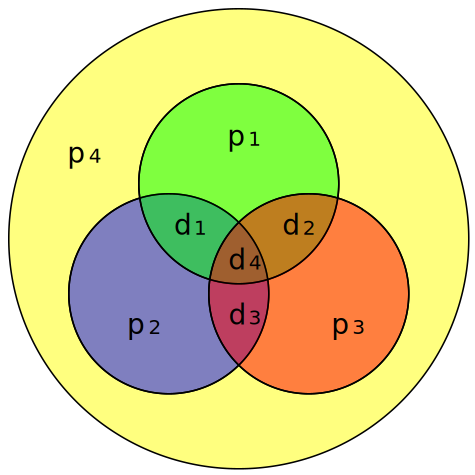
\includegraphics[width=0.4\textwidth]{images/hamming8.4.png}
    \caption{8,4 Hamming Code}
\end{figure}

\href{https://www.youtube.com/watch?v=X8jsijhllIA}{3B1B Hamming Codes Video}

\subsection{Bildkodierung}

Bei einem Bild wird die Farbe eines Pixel Grundsätzlich durch 3 Werte, einen Rot,
Grün und Blau Wert festgelegt und so gespeichert. Diese Werte können dabei jeweils
8, 10, 16 oder mehr Bit groß sein, wodurch sich der Farbraum der Pixel vergrößert.
Zusätzlich kann noch die Transparenz eines Pixels gespeichert werden, der Alpha Wert.
Je nach Bitanzahl pro Pixel und Kompression unterscheiden sich so Bilder verschiedener
Qualitäten und Formate (e.g. JPG, PNG). Meist werden Bilder mit 8 Bit Werten gespeichert,
also 8 Bit jeweils für Rot, Grün, Blau. Jede Farbe hat somit einen Wert zwischen 0 und 255.
Ein Pixel kann also $255^3$ unterschiedliche Farben annehmen. Das sind ca. 16,7 Millionen
Farben.

\begin{figure}[H]
    \centering
    \includegraphics[width=0.8\textwidth]{images/rgbvalues.png}
    \caption{Verschiedene Farbtiefen bei Bildern}
\end{figure}

\section{Objektorientierung}
\subsection{Klassen}

Die Objektorientierte Programmierung mit Klassen hat zum Ziel,
reale Zusammenhänge zu modellieren und Dinge zu strukturen und
zu organisieren. Dazu gibt es Klassen mit Attributen und Methoden
mit denen sich Objekte (Instanzen der Klasse) erzeugen lassen.
Eine Klasse ist ein Schemata zur Erzeugung eines Objekts.

\pgfsetlayers{package0, main}

\vspace*{0.5cm}
\begin{figure}[H]
\begin{center}
\hspace*{-2cm}
\begin{minipage}{.7\textwidth}
    \begin{lstlisting}[language=python]
    class Car:
        def __init__(self, name: str, speed: float):
            self.name = name      # Attribut
            self.speed = speed
            self.__km_driven = 0
            
        def getDriven() -> float: # Methode
            return self.__km_driven
            
        def drive(hours: float):
            self.__km_driven += self.speed * hours
    \end{lstlisting}
    \caption{Klasse in Python}
\end{minipage}
\begin{minipage}{.3\textwidth}
    \begin{tikzpicture}
        \umlclass{Auto}{ 
        + name : Zeichenkette \\ 
        + speed : Dezimalzahl \\ 
        - km\_driven : Dezimalzahl
        }{ 
            + getDriven() : Dezimalzahl \\
            + drive(hours: Dezimalzahl) :
            }
    \end{tikzpicture}
    \caption{UML Klassendiagramm}
\end{minipage}
\end{center}
\end{figure}

\subsection{Vererbung}
\subsection{Klassendiagramme}
\section{Datenbanken}

\subsubsection{Begriffe bei Datenbanken}

<Todo: Primärschlüssel, attribut, fremschlüssel, tabelle, einfüge, änderungs, löschanomalie>


\subsection{Entity-Relationship-Modelle (ER-Modelle)}

Ein Entity-Relationsip Modell soll Entitäten und Beziehungen eines Sachverhalts
darstellen und so z. B. die Erstellung einer Datenbank erleichtern.
Es gibt mehrere Arten zur Notation von Entity Relationship Modellen,
in diesem Fall wird die Chen Notation betrachtet.

\vspace*{1cm}

\adjustbox{scale=0.8}{
\begin{tikzpicture}[auto,node distance=1cm]
\node[entity] (node1) {Student}[grow=up,sibling distance=3.5cm]
    child[text width=2cm, align=center, level distance=2cm] {node[attribute] {Lastname}}
    child[text width=2cm, align=center, level distance=2cm] {node[attribute] {Firstname}}
    child[text width=2cm, align=center, level distance=2cm] {node[attribute] {\underline{ID}}};

\node[relationship] (rel1) [below = of node1] {Takes};
\node[attribute] (node4) [left = of rel1] {Hours};
\path (rel1) edge (node4);

\node[entity] (node2) [below = of rel1]{Class}[grow=down,sibling distance=3.5cm]
    child[text width=2cm, align=center, level distance=2cm] {node[attribute] {\underline{ID}}}
    child[text width=2cm, align=center, level distance=2cm] {node[attribute] {Subject}}
    child[text width=2cm, align=center, level distance=2cm] {node[attribute] {Teacher}};
\path (rel1) edge node {n} (node1) edge node {m}(node2);

\node[relationship] (rel2) [right = of node1] {Goes To};

\node[entity] (node3) [right = of rel2]{School}[grow=right, sibling distance=2.5cm]
    child[text width=2cm, align=center, level distance=2cm] {node[attribute] {\underline{ID}}}
    child[text width=2cm, align=center, level distance=2cm, xshift=2cm] {node[attribute] {Name}}
    child[text width=2cm, align=center, level distance=2cm] {node[attribute] {Type}};

\path (rel2) edge node {m} (node1) edge node {1}(node3);
\end{tikzpicture}
}

\vspace*{0.3cm}

\subsubsection{Erklärung der ER-Notation nach Chen}

\vspace*{0.3cm}

\begin{enumerate}
    \item Ein Rechteck stellt eine Entität dar.
    \item Ein Oval stellt ein Attribut einer Entität dar.
    \item Ein unterstrichenes Attribut ist Teil des Primärschlüssels.
    \item Eine Raute erläutert die Beziehung zweier Entitäten.
    \item Ein Oval an einer Raute kann der Beziehung Attribute zuordnen.
    \item An einer Beziehung zwischen zwei Entitäten sind die Kardinalitäten notiert.
\end{enumerate}

\clearpage

\subsubsection{Kardinalitäten}

Die Kardinälität einer Beziehung beschreibt, wie vielen Entitäten der anderen
Entität zugeordnet werden können. Beispielsweise kann ein Schüler nur auf 1 Schule 
gehen, aber auf eine Schule können viele Schüler gehen. Klassen besucht ein Schüler
hingegen mehrere und in eine Klasse gehen mehrere Schüler. Es gibt folgende Kardinalitäten,
wobei man bei jeder Kardinalität auch angeben kann, ob einer Zuordnung optional ist
oder wie viele Zuordnung es geben muss.

\begin{table}[H]
    \begin{tabular}{|l|l|l|}
    \hline
        Kardinälität & Entität A & Entität B \\ \hline
        Eins zu Eins & 1 & 1 \\ \hline
        Eins zu Vielen & 1 & m \\ \hline
        Viele zu Eins & m & 1 \\ \hline
        Viele zu Viele & m & n \\ \hline
        \end{tabular}
\end{table}

\subsection{Normalformen}

Bei der Erstellung eines Datenbankschemas in einer Relationellen Datenbank
(z. b. aus einem ER-Modell) unterscheidet man, je nach Eigentschaften des
Schematas, in welcher Normalform sich dieses befindet. Ein Schemata kann
von einer Normalform in eine andere (nächthöhere) überführt werden.
Dies lässt sich auch automatisiert durchführen. Jede dieser Normalformen
unterscheidet sich darin, wie die Abhängigkeiten zwischen den Tabellen
und Attributen sind. Je höher die Normalform, desto weniger Redundanz der Daten
(Wiederholung) ist vorhanden und desto weniger Inkosistenz und Anomalien gibt es.

\subsubsection{0. Normalform}

Die Daten liegen unstrukturiert, redundant und nicht-atomar vor.

\newcolumntype{a}{>{\columncolor{blue!20}}l}
\newcolumntype{d}{>{\columncolor{yellow!50}}l}

\begin{table}[H]
    \begin{tabular}{|a|l|l|l|}
    \hline
        CD\_ID & Albumtitel & Gründungsjahr & Titelliste \\ \hline
        11 & Sniff Dog - Los Angeles & 1995 & {1. Crazy 2. Love 3. Crack} \\ \hline
        12 & Jay-X - Goodbye New York & 1965 & {1. Imperial State of Math} \\ \hline
        13 & Sniff Dog - Dr. Drug & 1999 & {1. Weed Every Day} \\ \hline
    \end{tabular}
\end{table}

\clearpage

\subsubsection{1. Normalform}

Die Anforderungen an die 1. NF sind, dass alle Attribute atomar sind und
unnötige Spalten und Daten zusammengefasst werden, ohne das Informationen verloren gehen.

\begin{table}[H]
    \begin{tabular}{|a|l|l|l|a|l|}
    \hline
        CD\_ID & Albumtitel & Interpret & Gründungsjahr & Track & Titelliste \\ \hline
        11 & Los Angeles & Sniff Dog & 1993 & 1 & Crazy \\ \hline
        11 & Los Angeles & Sniff Dog & 1993 & 2 & Love \\ \hline
        11 & Los Angeles & Sniff Dog & 1993 & 3 & Crack \\ \hline
        12 & Goodbye New York & Jay-X & 1965 & 1 & Imperial State of Math \\ \hline
        13 & Dr. Drug & Sniff Dog & 1993 & 1 & Weed Every Day \\ \hline
    \end{tabular}
\end{table}

\subsubsection{2. Normalform}

Die Anforderungen an die 2. NF sind die an alle Vorigen und dass keine
nicht-schlüssel Attribute in einer Relation nur von einem Teil des Primärschlüssels
abhängig sind (jedes Attribut einer Relation ist voll funktional abhängig vom Primärschlüssel dieser).

\begin{table}[H]
    \begin{tabular}{|a|l|l|l|}
    \hline
        CD\_ID & Albumtitel & Interpret & Gründungsjahr \\ \hline
        11 & Los Angeles & Sniff Dog & 1993 \\ \hline
        12 & Goodbye New York & Jay-X & 1965 \\ \hline
        13 & Dr. Drug & Sniff Dog & 1993 \\ \hline
    \end{tabular}
\end{table}

\begin{table}[H]
    \begin{tabular}{|a|a|l|}
    \hline
        CD\_ID & Track & Titel \\ \hline
        11 & 1 & Crazy \\ \hline
        11 & 2 & Love \\ \hline
        11 & 3 & Crack \\ \hline
        12 & 1 & Imperial State of Math \\ \hline
        13 & 1 & Weed Every Day \\ \hline
    \end{tabular}
\end{table}

\clearpage

\subsubsection{3. Normalform}

Die Anforderungen an die 3. NF sind die an alle Vorigen und dass keine
nicht-schlüssel Attribute in einer Relation von anderen nicht-schlüssel Attributen
funktional abhängegen. Diese nicht gewollten Abhängigkeiten nennt man transistive Abhängigkeiten.

\begin{table}[H]
    \begin{tabular}{|a|l|d|}
    \hline
        CD\_ID & Albumtitel & Interpret\_ID \\ \hline
        11 & Los Angeles & 21 \\ \hline
        12 & Goodbye New York & 22 \\ \hline
        13 & Dr. Drug & 21 \\ \hline
    \end{tabular}
\end{table}

\begin{table}[H]
    \begin{tabular}{|a|l|l|}
    \hline
        Interpret\_ID & Interpret & Gründungsjahr \\ \hline
        21 & Sniff Dog & 1993 \\ \hline
        22 & Jay-X & 1965 \\ \hline
        21 & Sniff Dog & 1993 \\ \hline
    \end{tabular}
\end{table}

\begin{table}[H]
    \begin{tabular}{|a|a|l|}
    \hline
        CD\_ID & Track & Titel \\ \hline
        11 & 1 & Crazy \\ \hline
        11 & 2 & Love \\ \hline
        11 & 3 & Crack \\ \hline
        12 & 1 & Imperial State of Math \\ \hline
        13 & 1 & Weed Every Day \\ \hline
    \end{tabular}
\end{table}

\clearpage

\subsection{SQL}
\subsubsection{Struktur von SQL Abfragen}

\section{Kryptologie}
\subsection{Verschlüsselung im Alltag}

Verschlüsselung ist ein Grundpfeiler der modernen Kommunikation und absolut nötig,
damit kein Unbekannter und Unbefugter private Nachrichten oder Passwörter mitlesen
kann. Ohne starke Verschlüsselungsverfahren wäre die weitergabe sensibler Daten über
das Internet nicht möglich.

\subsection{Historische Verschlüsselungsverfahren}

\subsubsection{Caesar Chiffre}

Schon die alten Römer und viele nach ihnen erkannten, dass es durchaus von Vorteil
ist, wenn die Feinde nichts über den geheimen Schlachtplan oder die nächste Intrige
erfahren können.
Das sogenannte Caesar-Chiffre ist die einfachste Form eines symetrischen,
monoalphatischen Verschlüsselungsverfahren für Texte.
Man bestimmt eine Verschiebung zwischen 1 und 25 und ersetzt dann
alle Buchstaben des Klartexts, um den Geheimtext zu erhalten.
Kennt man die Verschiebung, so lässt sich die Nachricht auch wieder entschlüsseln.
Dieses Verfahren ist allerdings nicht sicher, weswegen es heutzutage niemand verwendet.
Um einen Buchstaben zu verschlüsseln sucht man diesen im oberen Alphabet und
ersetzt diesen dann durch den Buchstaben darunter aus dem unteren Alphabet.
Beim Entschlüsseln ist dies umgekehrt. Man ersetzt den Buchstaben im Geheimtext
durch den Buchstaben aus dem oberen Alphabet, der über der Position des Buchstabens
im unteren Alphabet ist.

\begin{lstlisting}
A B C D E F G H I J K L M N O P Q R S T U V W X Y Z
Y Z A B C D E F G H I J K L M N O P Q R S T U V W X

Klartext:     INFORMATIK
Geheimtext: GLDMPKYRGI
\end{lstlisting}

\clearpage

\subsection{Symetrische Verschlüsselung}

Symetrische Verschlüsselungsverfahren zeichnen sich dadurch aus, dass zum
Ent- und Verschlüsseln der gleiche Algorithmus und der gleiche Schlüssel verwendet
wird. Beispiele sind die Caesar Chiffre, die Vigenere Chriffe oder das Blockchiffre AES-256.

\subsubsection{Blockchriffen}

Blockchiffre Verfahren sind symetrische Verschlüsselungsverfahren,
die auch zur Verschlüsselung größerer Datenmengen genutzt werden können.
Eine besondert dieser ist, dass die zu verschlüsselnden Daten Blockweise
verschlüsselt werden und in die Verschlüsselung eines Block das Ergebnis
der Verschlüsselung des vorigen Blocks mit eingeht.
Blockchiffren wie Advanced Encryption Standard (AES) mit hohen Bitlängen (e.g. AES-256)
sind mit heutigen Mitteln unknackbare Verfahren, weswegen diese breite Anwendung
z. B. bei Datenübertragung oder Festplattenverschlüsselung finden.

\subsubsection{Diffie-Hellman Verfahren}

Dieses von Whitfield Diffie und Martin Hellman entwickelte Verfahren ermöglicht es,
dass zwei Kommunikationspartner einen gemeinsamen, geheimen Schlüssel in Form einer Zahl
vereinbaren, auch wenn ihre Kommunikationsleitung öffentlich (unverschlüsselt ist).
Dadurch lassen sich einfach Schlüssel austauschen, um danach z. B. die Kommunikation
mit AES zu verschlüsseln.

\begin{lstlisting}
a: 0 < natürliche Zahl < p
b: 0 < natürliche Zahl < p
p: öffentliche Primzahl
g: 0 < öffentliche natürliche Zahl < p
A: öffentliche Schlüssel Alice
B: öffentliche Schlüssel Bob
K: geheimer Schlüssel, nur Bob und Alice bekannt
\end{lstlisting}

\begin{figure}[H]
    \centering
    \includegraphics[width=0.6\textwidth]{images/diffie-hellman.png}
    \caption{\textbf{Diffie-Hellman Schlüsseltausch}}
\end{figure}

\clearpage

\subsection{Asymetrische Verschlüsselung (Public Key Cryptography)}

Die asymetrische Verschlüsselung zeichnet sich im Unterschied zur symetrischen
Verschlüsselung dadurch aus, dass es 2 Schlüssel gibt. Den einen zum Ver-, den anderen
zum Entschlüsseln. Diese beiden Schlüssel nennt man ein Schlüsselpaar.

\subsubsection{Schlüsselpaare}
Es gibt verschiedene Algorithmen, um kryptographische Schlüsselpaare zu erstellen.
Die bekanntesten und besten sind RSA und EdDSA und Variationen dieser.
Je nach Verfahren kann die Bitlänge der Schlüssel variieren, wobei höhere Bitlängen
sicherer sind. Die eigenschaften des Schlüsselpaars sind wie folgt.

\begin{lstlisting}
privater Schlüssel (öffentlicher Schlüssel (Nachricht)) = Nachricht
öffentlicher Schlüssel (privater Schlüssel (Nachricht)) = Nachricht 
\end{lstlisting}

\subsubsection{Verschlüsselung mit Public und Private Key}

Beide Kommunikationspartner erstellen ein asymetrisches Schlüsselpaar.
Anschließend übertragen beide den öffentlichen Schlüssel an den Kommunikationspartner.
Nun können Nachrichten mit dem öffentlichen Schlüssel des Partners verschüsselt werden
und nur dieser kann diese mit dem privaten Schlüssel entschlüsseln. Niemand sonst kann
so die Kommunikation mitverfolgen. Es ist auch möglich, nun auf diesem verschlüsselten
Kanal einen symetrischen Schlüssel auszutauschen und z. B. AES-256 in der weiteren
Kommunikation zu verwenden.

\begin{figure}[H]
    \centering
    \includegraphics[width=0.5\textwidth]{images/public-key-encryption.png}
    \caption{\textbf{Verschlüsselung mit Schlüsselpaaren}}
\end{figure}

\clearpage

\subsection{Digitale Signaturen}

\subsubsection{Das Authentizitätsproblem}

Wenn Alice und Bob ihre Schlüssel ausgetauscht haben, kann niemand ihre Nachrichten mitlesen.
Doch fängt jemand jeweils die öffentlichen Schlüssel von Bob und Alice bei der Übertragung ab,
so kann diese Person den Beiden Nachrichten schicken, von denen diese denken, sie wärem vom
jeweils anderen.

\subsubsection{Lösung mit digitalen Signaturen und Hash-Werten}

Damit Alice und Bob sicher sein können, dass niemand ihre Nachrichten verändert oder
ihnen Falschnachrichten sendet, können diese ihre Nachrichten mit ihren Schlüsseln signieren.
Anstatt ihre Nachricht nur mit Bobs öffentlichem Schlüssel zu verschlüsseln, wendet Alice vorher noch
ihren Privaten Schlüssel auf die Nachricht an. Jede Person mit Alice öffentlichem Schlüssel
kann so feststellen, dass die Nachricht von ihr kommt. Würde man diese Nachricht mit Alice
öffentlichem Schlüssel entschlüsseln wollen, und es wäre ein anderer privater Schlüssel
verwendet worden (z. B. von Eve), so würde sich keine Nachricht ergeben und man wüsste,
dass diese Nachricht nicht von Alice sein kann. Anschließend verschlüsselt sie wie vorher
auch die Nachricht mit Bobs öffentlichem Schlüssel, da diese sonst jeder mitlesen könnte.
Nur Bob kann nun die Nachricht entschlüsseln und anschließend kann er mit Alice öffentlichem
Schlüssel die Authentizität überprüfen. Nun kann niemand anderes Bob Nachrichten in Alice Namen
senden. Gleiches gilt nun natürlich auch für Alice.

\begin{lstlisting}[basicstyle=\small]
PubKeyBob (PrivKeyAlice (Alice Nachricht)) = Alice Nachricht verschlüsselt und signiert
PrivKeyBob (Alice Nachricht verschlüsselt und signiert) = Alice Nachricht signiert
PubKeyAlice (Alice Nachricht signiert) = Nachricht
\end{lstlisting}

Ist Alice Nachricht sehr groß und sie will nicht auf die komplette Nachricht
ihren privaten Schlüssel anwenden (z. B. aus Effizienzgründen), so kann sie
einen Hash-Wert (dieser ist deutlich kürzer als die Nachricht) der Nachricht erstellen
und nur diesen signieren. Anschließend verschlüsselt sie dann die Nachricht und
den signierten Hash-Wert und schickt diese an Bob.
Bob weiß, dass nur Alice ihm diesen Hash-Wert übermittelt haben kann, und kann so
prüfen, ob der Hash-Wert zur Nachricht passt, also ob die Nachricht wirklich von Alice
ist. Dazu nutzt er die gleiche Hash-Funktion wie Alice und prüft, ob sein und der signierte
Hash-Wert der gleiche sind.

\subsubsection{Erklärung von Hash-Funktionen und Hash-Werten}

Eine Hash-Funktion erstellt zu einer Eingabe an Daten einen Hash-Wert fester Länge.
Für die gleichen Daten ist dieser Hash-Wert beim mehrmaligen ausführen der 
Funktion auf diese Daten immer gleich.
Bei einer guten, kryptographisch sicheren Hash-Funktionen haben nahezu nie verschiedene
Daten den gleichen Hash-Wert und eine Umkehr der Funktion ist nicht einfach möglich.
Dadurch wird verhindert, dass man zu einem Hash-Wert einfach die Daten finden kann, die
diesen erzeugen.

\subsection{Zertifikate}

\subsubsection{Das Integritätsproblem}

Jetzt schaltet sich jedoch Eve dazwischen und startet einen Man-in-the-Middle Angriff.
Sie fängt die öffentlichen Schlüssel von Bob und Alice bei der Übertragung
ab und ersetzt diese durch einen öffentlichen Schlüssel eines anderen Schlüsselpaars (links).
Da Eve dazwischen geschaltet ist, kann sie jede Nachricht nun abfangen, entschlüsseln, lesen
und verändern (rechts). Anschließend sendet sie die Nachricht mit dem abgefangenen, echten öffentlichen
Schlüssel weiter an Bob bzw. Alice. Auch eine digitale Signatur von Alice auf die ganze Nachricht bringt nichts,
da Eve diese entschlüsseln kann und dann mit ihrem privaten Schlüssel eine neue
Signatur für Bob erstellt.

\vspace*{0.5cm}

\begin{center}
\adjustbox{scale=1.0}{
\begin{tikzpicture}
% left %
% alice
\draw (0,0) rectangle (4,2);
\node[draw] at (2,1.5) {Alice};
\node[draw=red, thick, rounded corners, fill=red!20] at (1,0.7) {Pub};
\node[draw=red, thick, rounded corners, fill=red!20] at (3,0.7) {Priv};
% eve
\draw (0,4) rectangle (4,6);
\node[draw] at (2,5.5) {Eve};
\node[draw=violet, thick, rounded corners, fill=violet!20] at (1,4.7) {Pub};
\node[draw=violet, thick, rounded corners, fill=violet!20] at (3,4.7) {Priv};
% bob
\draw (0,8) rectangle (4,10);
\node[draw] at (2,9.5) {Bob};
\node[draw=green, thick, rounded corners, fill=green!20] at (1,8.7) {Pub};
\node[draw=green, thick, rounded corners, fill=green!20] at (3,8.7) {Priv};
% arrows
\draw [-{Latex[length=2mm]}] (1,4) -- (1,2);
\draw [-{Latex[length=2mm]}] (3,2) -- (3,4);
\draw [-{Latex[length=2mm]}] (1,8) -- (1,6);
\draw [-{Latex[length=2mm]}] (3,6) -- (3,8);
% labels
\node[draw=red, thick, rounded corners, fill=red!20] at (3,3) {Pub};
\node[draw=violet, thick, rounded corners, fill=violet!20] at (1,3) {Pub};
\node[draw=violet, thick, rounded corners, fill=violet!20] at (3,7) {Pub};
\node[draw=green, thick, rounded corners, fill=green!20] at (1,7) {Pub};

% right %
% alice
\draw (6,0) rectangle (10,2);
\node[draw] at (8,1.5) {Alice};
\node[draw=red, thick, rounded corners, fill=red!20] at (7,0.7) {Priv};
\node[draw=violet, thick, rounded corners, fill=violet!20] at (9,0.7) {Pub};
% eve
\draw (6,4) rectangle (10,6);
\node[draw] at (8,5.5) {Eve};
\node[draw=red, thick, rounded corners, fill=red!20] at (6.8,4.6) {Pub};
\node[draw=violet, thick, rounded corners, fill=violet!20] at (6.8,5.4) {Priv};
\node[draw=violet, thick, rounded corners, fill=violet!20] at (9.2,4.6) {Priv};
\node[draw=green, thick, rounded corners, fill=green!20] at (9.2,5.4) {Pub};
% bob
\draw (6,8) rectangle (10,10);
\node[draw] at (8,9.5) {Bob};
\node[draw=violet, thick, rounded corners, fill=violet!20] at (7,8.7) {Pub};
\node[draw=green, thick, rounded corners, fill=green!20] at (9,8.7) {Priv};
% arrows
\draw [red, -{Latex[length=2mm]}] (7,4) -- (7,2);
\draw [violet, -{Latex[length=2mm]}] (9,2) -- (9,4);
\draw [violet, -{Latex[length=2mm]}] (7,8) -- (7,6);
\draw [green, -{Latex[length=2mm]}] (9,6) -- (9,8);

\end{tikzpicture}
}
\end{center}

\clearpage

\subsubsection{Lösung mit Zertifikaten und Zertifikatsstellen}

Bob hat eine Bank gegründet, bei der Alice Kundin ist. Damit Eve ihre vertrauliche Kommunikation
nicht mithören kann, nutzt Bob ein Zertifikat für seine Bank.
Nachdem Bob sein Schlüsselpaar generiert hat, hat er bei der Zertifikatsstelle ein Zertifikat
beantragt. Dazu musste er sich bei einer Zertifikatsstelle authentifizieren und zeigen, dass er
wirklich der Betreiber von Bob's Bank ist. Anschließend hat die Zertifikatsstelle ein
Zertifikat für seine Bank erstellt, in welchem sein öffentlicher Schlüssel sowie Informationen
über seine Bank mit dem privaten Schlüssel der Zertifizierungsstelle signiert ist.
Dieses sendet Bob nun an Alice, um zu bestätigen, dass sie wirklich mit Bob's bank kommuniziert.
Alice kann die Signatur des Zertifikats prüfen, da sie im voraus den öffentlichen Schlüssel
von der Zertifikatsstelle erhalten hat. Sie weiß dann, ob sie wirklich Bob's öffentlichen
Schlüssel erhalten hat. Eve kann kein Zertifikat für Bob's Bank beantragen, da sie sich
dafür bei der Zertifizierungsstelle als Bob authentifizieren müsste.
Beantragt sie ein anderes Zertifikat, so erkennt Alice, dass dieses nicht für Bob's Bank,
sondern für jemand anderen ausgestellt ist.
Erstellt Eve selbst ein Zertifikat, so erkennt Alice mit dem öffentlichen Schlüssel der
Zertifizierungsstelle, dass dieses gefälscht ist.
Dies funktioniert allerdings nur, weil Bob und Alice beide Faythe, dem Betreiber
der Zertifikatsstelle vertrauen und weil dieser sehr gewissenhaft arbeitet.
Da Alice Kundin bei Bob ist, kann sie sich über die gesichterte Verbindung nun mit ihrem
Password authentifizieren. Da sie den öffentlichen Schlüssel aus dem Zertifikat nutzt weiß sie,
dass nur Bob die Nachricht lesen kann.
Unter anderen Umständen, z. B. bei der Kommunikation zwischen Servern in einem Unternehmen
ist es auch möglich, dass diese sich gegenseitig Zertifikate zusenden.

\clearpage

\vspace*{2.5cm}

\begin{center}
\adjustbox{scale=1.4}{
\begin{tikzpicture}
% left %
\draw (-1,6) rectangle (4,8);
\node[draw] at (1,7.5) {Zertifikatsstelle};
\node[draw=yellow, thick, rounded corners, fill=yellow!20] at (0,6.7) {Pub};
\node[draw=yellow, thick, rounded corners, fill=yellow!20] at (3.3,6.7) {Priv};
% right %
% alice
\draw (6,0) rectangle (10,2);
\node[draw] at (8,1.5) {Alice};
\node[draw=red, thick, rounded corners, fill=red!20] at (7,0.7) {Priv};
\node[draw=red, thick, rounded corners, fill=red!20] at (9,0.7) {Pub};
\draw (6,-2.1) rectangle (10, -0.1);
\node[draw] at (8,-0.6) {Prüfschlüssel};
\node[draw=yellow, thick, rounded corners, fill=yellow!20] at (7,-1.4) {Pub};
% bob
\draw (6,7) rectangle (10,10);
\node[draw] at (8,9.5) {Bob's Bank};
\node[draw=green, thick, rounded corners, fill=green!20] at (7,8.7) {Pub};
\node[draw=blue, thick, rounded corners, fill=blue!20] at (7,7.7) {Cert};
\node[draw=green, thick, rounded corners, fill=green!20] at (9,8.7) {Priv};
% arrows
\draw [-{Latex[length=2mm]}] (9,2) -- (9,7);
\draw [-{Latex[length=2mm]}] (7,7) -- (7,2);
\node at (4.3, 9) {beantragt};
\draw [-{Latex[length=2mm]}] (6.45,8.7) -- (3.3, 8.7) -- (3.3, 7);
\node at (4.3, 3.7) {stellt aus};
\draw [-{Latex[length=2mm]}] (3.3, 6.4) -- (3.3, 4) -- (5.5, 4) -- (5.5, 7.7) -- (6.45, 7.7);
\node at (0.8, -1.7) {verteilt};
\draw [-{Latex[length=2mm]}] (0, 6.4) -- (0, -1.4) -- (6.45, -1.4);
% labels
\node[draw=blue, thick, rounded corners, fill=blue!20] at (7,4.5) {Cert};

\end{tikzpicture}
}
\end{center}

\section{Datenschutz}
\subsection{Grundbegriffe des Datenschutzes}
\subsection{Datenschutz-Grundverordnung (DSGVO)}

\end{document}
